\documentclass[tikz,border=6pt]{standalone}

\usepackage[T1]{fontenc}
\usepackage[utf8]{inputenc}
\usepackage{tikz}
\usetikzlibrary{arrows.meta,backgrounds,fit,positioning,calc}

\definecolor{COne}{RGB}{229,115,115}
\definecolor{CTwo}{RGB}{255,183,77}
\definecolor{CThree}{RGB}{129,199,132}
\definecolor{CFour}{RGB}{100,181,246}
\definecolor{PanelGray}{RGB}{247,248,250}

\tikzset{
  node base/.style={
    draw,
    circle,
    minimum size=5.8mm,
    inner sep=0pt,
    font=\scriptsize,
    thick
  },
  c1/.style={node base,fill=COne!26,draw=COne!75!black},
  c2/.style={node base,fill=CTwo!32,draw=CTwo!75!black},
  c3/.style={node base,fill=CThree!28,draw=CThree!75!black},
  c4/.style={node base,fill=CFour!28,draw=CFour!75!black},
  panel/.style={draw,rounded corners=5pt,fill=PanelGray,inner sep=5pt},
  title/.style={font=\footnotesize\bfseries},
  note/.style={draw,rounded corners=3pt,fill=white,align=center,font=\footnotesize,inner sep=4pt},
  bucket/.style={draw,rounded corners=2pt,minimum width=0.88cm,minimum height=0.46cm,font=\scriptsize,inner sep=2pt},
  subtle/.style={font=\scriptsize\itshape,text=gray!70!black},
  edge/.style={gray!70,thick},
  arrow/.style={-Latex,thick},
  highlight/.style={draw=gray!55,dashed,rounded corners=4pt}
}

\begin{document}
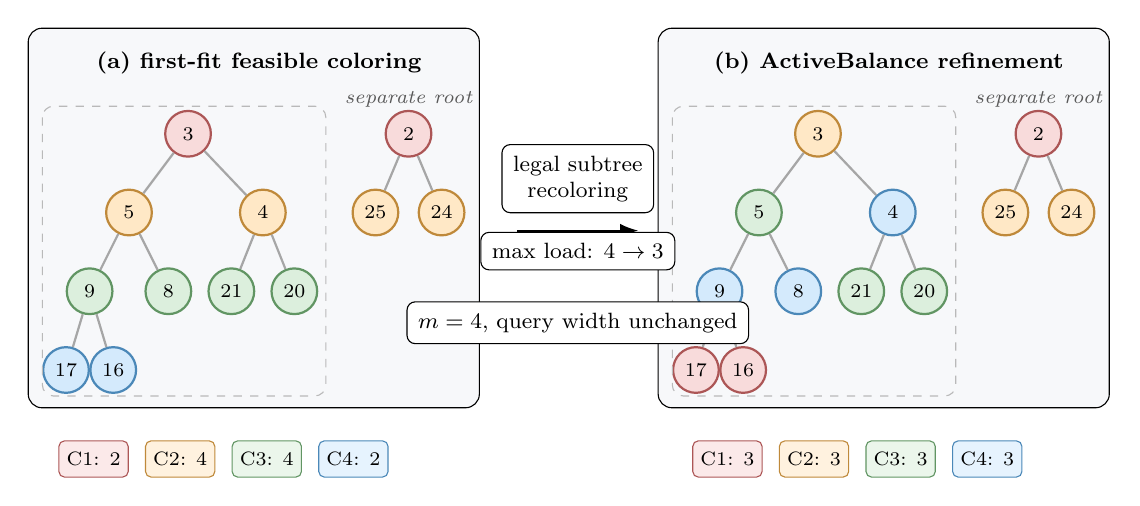
\begin{tikzpicture}[x=1cm,y=1cm]

% Left panel: first-fit feasibility coloring on the served-interval forest.
\node[title] (ltitle) at (-4.20,2.25) {(a) first-fit feasible coloring};
\node[c1] (l3) at (-5.10,1.35) {3};
\node[c1] (l2) at (-2.30,1.35) {2};
\node[c2] (l5) at (-5.85,0.35) {5};
\node[c2] (l4) at (-4.15,0.35) {4};
\node[c2] (l25) at (-2.72,0.35) {25};
\node[c2] (l24) at (-1.88,0.35) {24};
\node[c3] (l9) at (-6.35,-0.65) {9};
\node[c3] (l8) at (-5.35,-0.65) {8};
\node[c3] (l21) at (-4.55,-0.65) {21};
\node[c3] (l20) at (-3.75,-0.65) {20};
\node[c4] (l17) at (-6.65,-1.65) {17};
\node[c4] (l16) at (-6.05,-1.65) {16};

\draw[edge] (l3)--(l5);
\draw[edge] (l3)--(l4);
\draw[edge] (l5)--(l9);
\draw[edge] (l5)--(l8);
\draw[edge] (l9)--(l17);
\draw[edge] (l9)--(l16);
\draw[edge] (l4)--(l21);
\draw[edge] (l4)--(l20);
\draw[edge] (l2)--(l25);
\draw[edge] (l2)--(l24);
\draw[highlight] (-6.95,1.70) rectangle (-3.35,-1.98);
\node[subtle] at (-2.30,1.78) {separate root};

\node[bucket,fill=COne!16,draw=COne!75!black] at (-6.30,-2.78) {C1: 2};
\node[bucket,fill=CTwo!18,draw=CTwo!75!black] at (-5.20,-2.78) {C2: 4};
\node[bucket,fill=CThree!16,draw=CThree!75!black] at (-4.10,-2.78) {C3: 4};
\node[bucket,fill=CFour!16,draw=CFour!75!black] at (-3.00,-2.78) {C4: 2};

% Right panel: ActiveBalance refinement.
\node[title] (rtitle) at (3.80,2.25) {(b) ActiveBalance refinement};
\node[c2] (r3) at (2.90,1.35) {3};
\node[c1] (r2) at (5.70,1.35) {2};
\node[c3] (r5) at (2.15,0.35) {5};
\node[c4] (r4) at (3.85,0.35) {4};
\node[c2] (r25) at (5.28,0.35) {25};
\node[c2] (r24) at (6.12,0.35) {24};
\node[c4] (r9) at (1.65,-0.65) {9};
\node[c4] (r8) at (2.65,-0.65) {8};
\node[c3] (r21) at (3.45,-0.65) {21};
\node[c3] (r20) at (4.25,-0.65) {20};
\node[c1] (r17) at (1.35,-1.65) {17};
\node[c1] (r16) at (1.95,-1.65) {16};

\draw[edge] (r3)--(r5);
\draw[edge] (r3)--(r4);
\draw[edge] (r5)--(r9);
\draw[edge] (r5)--(r8);
\draw[edge] (r9)--(r17);
\draw[edge] (r9)--(r16);
\draw[edge] (r4)--(r21);
\draw[edge] (r4)--(r20);
\draw[edge] (r2)--(r25);
\draw[edge] (r2)--(r24);
\draw[highlight] (1.05,1.70) rectangle (4.65,-1.98);
\node[subtle] at (5.70,1.78) {separate root};

\node[bucket,fill=COne!16,draw=COne!75!black] at (1.75,-2.78) {C1: 3};
\node[bucket,fill=CTwo!18,draw=CTwo!75!black] at (2.85,-2.78) {C2: 3};
\node[bucket,fill=CThree!16,draw=CThree!75!black] at (3.95,-2.78) {C3: 3};
\node[bucket,fill=CFour!16,draw=CFour!75!black] at (5.05,-2.78) {C4: 3};

% Middle annotation
\draw[arrow] (-0.92,0.12) -- (0.62,0.12);
\node[note] at (-0.15,0.78) {legal subtree\\recoloring};
\node[note] at (-0.15,-0.14) {max load: $4 \rightarrow 3$};
\node[note] at (-0.15,-1.05) {$m=4$, query width unchanged};

\begin{pgfonlayer}{background}
  \node[panel,fit=(ltitle)(l3)(l2)(l17)(l16)(l24)(l25)] {};
  \node[panel,fit=(rtitle)(r3)(r2)(r17)(r16)(r24)(r25)] {};
\end{pgfonlayer}

\end{tikzpicture}
\end{document}
